\documentclass[12pt,a4paper]{article}
\usepackage[utf8]{inputenc}
\usepackage[russian]{babel}
\usepackage[OT1]{fontenc}
\usepackage{graphicx}
\usepackage[left=1cm,right=1cm,top=1cm,bottom=1cm]{geometry}
\author{Владимир Журавлев}
\usepackage{pgfplots}
\usepackage{graphicx}
\usepackage{amsmath}
\pgfplotsset{compat=1.9}
\pagestyle{plain}
\usepackage{pgfplotstable,filecontents}

\begin{document}
\begin{flushright}

\textbf{Журавлев Владимир, 621 гр.\\}


\end{flushright}
\begin{center}
\begin{LARGE}

\vspace{\baselineskip}
Лабораторная работа №4.3.4\\
\textbf{
ПРЕОБРАЗОВАНИЕ ФУРЬЕ В ОПТИКЕ}\\
\vspace{\baselineskip}

\end{LARGE}
\end{center}


\section{Определение ширины щели}
\subsection{Линза}
Для этого удобно использовать геометрическую оптику со значением волнового параметра $  \rho \ll 1$

Так же можно определить увеличение системы для линзы с фокусным расстоянием 
\[\Gamma = \frac{b}{a} \approx 23 \]
Построим график $D_\Gamma$ и $D_{exp}$:
\begin{center}
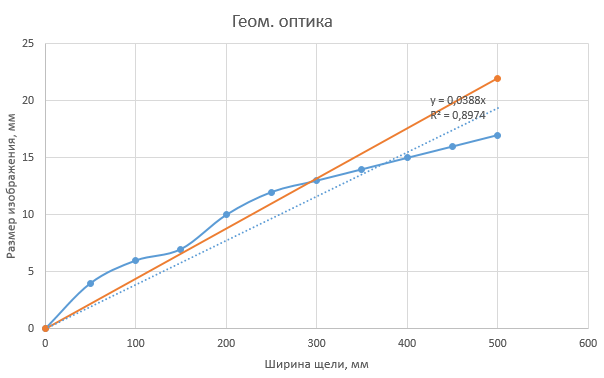
\includegraphics[scale=1]{434_g1.png}
\end{center}
\subsection{Спектр щели}
Используя соотношения для дифракции на щели:
\[\Delta X = \frac{X}{2m} = \frac{\lambda}{D_c} L\]
Можно найти ширину щели по дифракционной картине на экране.\\
Измерим все необходимое и построим график для обоих пунктов:

\begin{center}
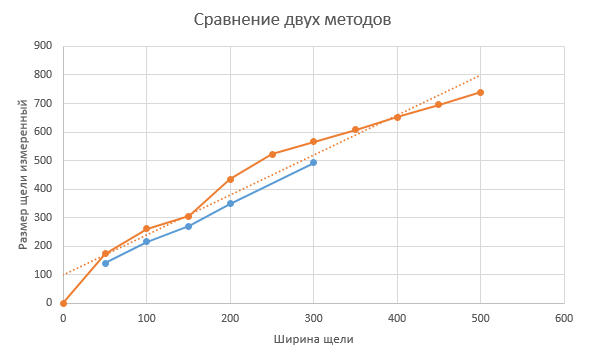
\includegraphics[scale=1]{434_g2.png}
\end{center}
Измерим ширину волоса:
\[ D_h  = \frac{2 \cdot 0.6328 \cdot1325}{20} \approx 70\; \mu m\]
\subsection{Определение периода решеток}

Определяя 
\[\Delta X = X/2m = \lambda L /d_c \]
\begin{center}
\begin{tabular}{|c|c|}
\hline 
N & $d_c$ \\ 
\hline 
1 & 22.7 \\ 
\hline 
2 & 34.0 \\ 
\hline 
3 & 68.4 \\ 
\hline 
4 & 299.45 \\ 
\hline 
5 & 342.22 \\ 
\hline 
\end{tabular} 

\end{center}
\subsection{Мультиплицирование}
Снимаем число промежутков между изображениями и расстояние между ними.
\[\Delta y = \frac{YK}{\gamma_2} \]
Построим график $\Delta y = f(1/d_c)$:\\

\begin{center}
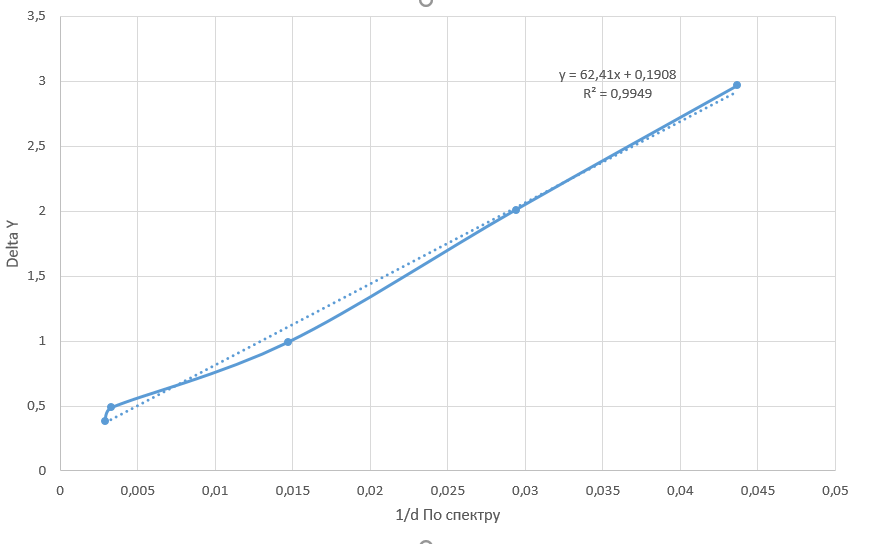
\includegraphics[scale=1]{434_g3.png}
\end{center}
\end{document}